\documentclass[10pt, oneside]{article}


\author{Philipp Jetzlaff}
\title{Projektdokumentation}

%%%%%%%%%%%%%%%%% P A C K A G E S %%%%%%%%%%%%%%%%%%%%%%%%%%%%%%%%%%%%%%%%%%%%%%%%%%%%%
%Package to create a custom header, that is printed on every page in the document.
\usepackage{fancyhdr}
%Package to include graphics.
\usepackage{graphicx}
\usepackage{helvet}
%Package to defines the paper enviroment
\usepackage[a4paper, headheight=60pt, bottom=20mm, left=25mm, right=25mm]{geometry}
%Package to defines hyperrefs in the document. E.g references to figures or tables
\usepackage{hyperref}
\usepackage{nameref}
%Packages to use sourcecode in this document
\usepackage{listings}
\usepackage{caption}

%Package to use colors in the documents. For example \rowcolor
\usepackage{color, colortbl}


%Define Header
\fancyhf{}
\fancyhead[R]{
\includegraphics[width=0.11\textwidth]{OktoPOS.png}}
\fancyhead[L]{
  \uppercase{Erweiterung eines Onlineserivce}\\
  \vspace{1pt}
  \small{Anbindung der OktoPOS Software an den internen Übersetzungsdienst}\\ 
  \vspace{4pt}
  \scriptsize{\leftmark}
}
\fancyfoot[L]{Philipp Jetzlaff}
\fancyfoot[R]{\thepage}
\renewcommand{\headrulewidth}{1pt}
\renewcommand{\footrulewidth}{1pt}
%Define Colors
\definecolor{LightCyan}{rgb}{0.88,1,1}
\definecolor{blue-green}{rgb}{0.0, 0.87, 0.87}
\definecolor{carolinablue}{rgb}{0.6, 0.73, 0.89}
\definecolor{lightgray}{rgb}{0.83, 0.83, 0.83}
%Define Codeblockfont
%Define imagepath
\graphicspath{{src/img/}}
%Define Listings apperiance
\lstset{basicstyle=\ttfamily}
%Overwrite naming for lists
\renewcommand{\listfigurename}{Abbildungsverzeichnis}
\renewcommand{\listtablename}{Tabellenverzeichnis}
\renewcommand{\contentsname}{Inhaltsverzeichnis}
%\renewcommand{\lstlistlistingname}{Listingsverzeichnis}
\renewcommand{\tablename}{Tabelle}
\renewcommand{\figurename}{Abbildung}
% Create new commands for work with refs.
\newcommand{\tabsecref}[1]{\hyperref[{#1}]{Tabelle \thesubsection. \nameref*{#1}}}
\newcommand{\figsecref}[1]{\hyperref[{#1}]{Abbildung \thesubsection. \nameref*{#1}}}
\newcommand{\attsecref}[1]{\hyperref[{#1}]{Anhang \thesubsection. \nameref*{#1}}}
\newcommand{\secref}[1]{\hyperref[{#1}]{\nameref{#1}}}
\newcommand{\tabref}[1]{\nameref{#1}}
\renewcommand{\familydefault}{\sfdefault}

\begin{document}
%Define Header and footer
  \pagestyle{fancy}
  
  %Deckblatt einfügen
  %table of contents
  \pagenumbering{roman}
  \tableofcontents
  \addcontentsline{toc}{section}{\listfigurename}
  \listoffigures
  \addcontentsline{toc}{section}{\listtablename}
  \listoftables
  \newpage
  \lstlistoflistings
  \newpage
  \section{Glossar}
  \newpage
  \pagenumbering{arabic}
  \section{Einleitung}%Überarbeiten
  !!!!! labels kontrollieren !!!!!
    ÜBERARBEITEN\\
    Im Rahmen der Abschlussarbeit für den Ausbildungberuft Fachinformatiker für Anwendungsentwicklung 
    wurde diese Projektdokumentation angefertigt. Sie dokumentiert den Ablauf und die Herangehensweise 
    welche zur Lösung, der im Vorfeld von dem zuständigen Ausbilder definierten, Aufgabe beigetragen haben. 
    Der Ausbildungsbetrieb OktoPOS Solutions GmbH ist ein mittelständiges Unternehmen mit Hauptsitz in Hamburg.
  \subsection{Projektbeschreibung}\label{sec:projectdesc}%Überarbeiten
    ÄNDERUNGEN HIER\\
    Das von der OktoPOS Solutions enwickelte Produkt OkotPOS Cash ist ein, im international Raum, genutztes POS System. 
    Für eine anwenderfreundliche Nutzung ist die gesamte Textausgabe des Front-End in diversen Sprachen konfigurierbar. 
    Zur Realisierung der Textausgabe in den geforderten Sprachen, werden im Quellcode Platzhalter (Tokens) statt konkreter Texte verwendet. 
    Für jede Sprache gibt genau eine Property Datei, in der die Texte der jeweiligen Sprache als Key-Value Paar hinterlegt sind.
    Die Erweiterung und Wartbarkeit dieser Property Dateien sind nach aktuellem Stand optimierungsbedürftig. 
    Es gibt keine Garantie dafür, dass jede Datei die selbe Anzahl an Tokens beinhalten bzw. es gibt keinen direkten Überblick 
    über den Übersetzungsstand der Dateien. 
    In den meisten Fällen werden die Übersetzungen von unternehmensfremden Personal angefertigt, 
    die mit der Struktur solcher Dateien nicht vertraut sind und daher mehr Zeit in Anspruch nehmen als notwendig.\\
    Der unternehmensinternen Übsersetzungsdienst TranslationService, bietet neben den grundlegenden Funktionen zum 
    Importieren/Exportieren von Tokens und Übersetzung auch ein benutzerfreundlichen Userinterface.
  \subsection{Projektziel}%Überarbeiten
    ÄNDERUNGEN HIER\\
    Ziel des Projektes ist es, durch die Anbindung der Kassensoftware an den unternehmensinternen Translationservice,
    den Prozess der Übersetzung von dem Releaseprozess zu entkoppeln und Versionsupdates der Übersetzungen während des Livebetriebes zu ermöglichen.
    Im Rahmen des Projektes soll die Integrität des Kassencodes erhalten bleiben. Deshalb ist es nötig den Updateprozess 
    in eine weitere Anwendung zu überführen. Die Anforderungen der Anwendung sind aus dem Soll-Konzept zu entnehmen.\\
    Der Transaltionservice ist zu so zu erweitern, dass Tokens und Übersetzungen in Abhängigkeit ihrer Version an den 
    Translationservice gesendet bzw. geladen werden können.
    Nach aktuellem Stand, ist der Translationservice nicht in der Lagen die Tokens und Übersetzungen zu Versionieren. 
    Das Anelgen einer neuen Version erfolgt von außen über eine zu schaffende Schnittstelle.Im Front-End des Translationservice, soll die Möglichkeit gegeben 
    werden die Tokens und den Stand der Übersetzung nach ihrer Version anzuzeigen.
    Da das Erstellen der Schnittstellen, die Implementierung der neuen Anwendung, das Testen der Komponenten usw. bereits die veranschlagten 70 Stunden benötigt,
    werden das Deployment der Minianwendung sowie die Anpasssung des Deploymentprozesses der Kassesoftware und die Anpassungen am Frontend als Fremdleistung an eine andere Abteilung weitergegeben. 
  \subsection{Projektumfeld}\label{sec:projectEnv}%Überarbeiten
    ÄNDERUNGEN HIER\\
    Primär ist das Projekt ein Auftrag der Entwicklungsabteilung des Kassensystems. Das Java gestützte POS System nutzt Übersetzungsdateien um Textstellen im Front-End in verschiedenen Sprachen darzustellen.
    Während der Entwicklung an der Kasse, speziell beim implementieren von Features, werden in machen Fällen neue Übersetzungstokens eingeführt. Der Entwickler muss dabei den Token in jede einzelne Datei schreiben. 
    Die Übersetzer des Tochterunternehmens OktoCareer nutzen den Translationserivce für die Übersetzungen an dem Personalmanagementsystem OktoCareer. 
    Der TranslationSerivce bietet eine Datenstruktur, welche mit geringen Aufwand auf die neuen Anforderungen angepasst werden kann, und die grundlegende Struktur für die RESTFull API. 
  \subsection{Projektabgrenzung}%Überarbeiten
    Die grundlegende Struktur des Translationservice ist bereits implementieren und wird produktiv im Betrieb genutzt. Das Projekt beschränkt sich hinsichtlich der Arbeiten an dem Transaltionservice nur auf das Hinzufügen der 
    neuen Schnittstellen, dem Erweiteren der Datenbank und den daraus resultierenden Änderungen an den vorhandenen Entitäten und Front-End Anpassungen.
    Durch die beschränkte Dauer die für dieses Projekt zur Verfügung gestellt wurde, hat zur Folge, dass Teile zur Realisierung des Gesamtprojektes an andere Abteilungen ausgelagert werden müssen.
    Dazu gehört der GitWebhook, welcher die Übersetzungsdateien der Kasse an den Übersetzungsdienst übergibt.
  \section{Projektplanung}
  \subsection{Projektphasen}%Überarbeiten
    Im Vorfeld des Projektes wurden die zu Verfügung stehenden 70 Entwicklerstunden auf verschiende Projektphasen aufgeteilt. 
    Die Zeiteinteilung sowie die einezlene Projektphasen wurden in einer groben Tabelle (\hyperref[tab:timing]{Tabelle 1: Grobe Zeiplanung}) zusammengefasst.
    Eine genaue Zeitplanung inklusive der Aufgaben jeder einzelnen Phase können aus dem \attsecref{sec:detailTime} entnommen werden. 
    \begin{table}[ht]
      \label{tab:timing}
      \centering
    \begin{tabular}{| l | r |}
      \hline
      \rowcolor{carolinablue}
      Projektphase & Stunden \\
      \hline
      Analysephase & 7h \\
      \hline
      \rowcolor{lightgray}
      Entwurfsphase & 11h\\
      \hline
      Implementierungsphase & 35h\\
      \hline
      \rowcolor{lightgray}
      Abnahme und Testphase & 3h\\
      \hline
      Dokumentation & 14h \\
      \hline
      \rowcolor{carolinablue}
      Gesamtstunden & 70h\\
      \hline
    \end{tabular}
    \caption{Grobe Zeitplanung}
  \end{table}
    Um die zeitliche Abfolge der einzelnen Projektphase grafisch darzustellen, wurden die einzelnen Aufgaben aus den 
    Projektphasen in sinngemäße Aufgaben zusammengefasst und ein Gantt-Chart überführt \attsecref{sec:GanttChart}.
  \subsection{Vorgehensmodel}%NOCH MACHEN
    ÄNDERUNGEN HIER
  \subsection{Resourcenplanung}%Überarbeiten
    Das Projekt wurde auf den von dem Ausbildungsbetrieb zur Verfügung gestellten Windows Surface Book und Windwos 10 geplant, bearbeitet und getestet. 
    Dabei wurde als Entwicklungsumgebung für den TransaltionService sowie für die Java App die für den Betrieb linzensierte 
    Software IntelliJ Ultimate von der Firma JetBrains verwendet. 
    Die Grundlage der Daten für den TranslationSerivce sind in einer MySql Datenbank gespeichert. 
    Zur Überprüfung der korrekten Anwendung des ORM Frameworks "Doctrine" hinsichtlich DDL und DQL, 
    wurden die Ergebnisse über die Software MySQL Workbench mittels SQL Abfragen validiert. 
    Neben den automatisierten Tests der Schnittstellen mit PHPUnit, 
    wurden regelmäßig mit der Software Postman Anfragen an die REST Schnittstellen geschickt.
    Für die, in Latex erstellte, Dokumentation notwendigen Diagramme wurden über den Onlinedienst Lucidchart angefertigt.
    Eine genaue Übersicht aller verwendeten Resoucren ist in der \attsecref{sec:resources} zu finden.
  \section{Analysephase}
  \subsection{Ist-Analyse}\label{sec:analyse:current}%Überarbeiten
    In der nachfolgende Analyse wird das Kassensystem OktoPOS Cash und der Übersetzungsdienst TranslationService in sein ursprünglichen Verfassung beschreiben.
  \subsubsection{OkotoPOS Cash}\label{sec:analyse:current:cash}%Überarbeiten
    Wie in der \secref{sec:projectdesc} und dem \secref{sec:projectEnv} beschrieben untertützt das Kassensystem OktoPOS Cash ein multilinguales Front-End.
    Um das zu gewährleisten, werden im Quellcode der Kasse s.g. Übersetzungstokens verwendent. Für jede unterstützte Sprache, ist eine Übersetzungs-datei im Porpertyformat
    in der Ressourcen der Kasse hinterlegt. Jede Datei beinhaltet das gleiche Set an Tokens mit der jeweiligen Übersetzung als Key-Value Paar. 
    Bei der Einführung eines neue Tokens kopiert der  Entwickler den neuen Token in eine der Dateien mit einer sinngemäßen Übersetzung.
    Da es im Unternehmen gängig ist, die Tokens nur in eine bzw. maximal zwei Datein zu überführen, wird die Aufgabe der Wartung und Pflege an 
    die Übersetzungsabteilung deligiert. Neben der trivialen und zeitaufwändigen Arbeit die einzelenen Dateien auf den gleich Stand zu halten
    kann es, auf Grund von diversen Faktoren, passieren das der Stand der Dateien divergiert.\\
    Bisher gibt es keine konkrete Oberfläche um Übersetzungen für die einzelnen Tokens anzufertigen bzw. auch keine direkte Refferenz auf die Textstelle 
    auf die der Token zeigen soll. Der Übersetzer hat die Aufgabe aus geeigneten Quellen (Ticketsystem, andere Übersetzungsdatei, Entwickler fragen) sich eine exemplarische Übersetzung
    zu beschaffen. Es gibt allerdings auch Fälle bei denen bisher keine Übersetzung für einen Token erstellt wurde. Dann hat der Übersetzer die Aufgabe, 
    über das Lesen von Quellcode die richtige Textstelle im Front-End zu finden.\\
    Im aktuellen Workflow werden die Übersetzungsdatein im Betazustand einer neuen Minorversion an die Abteilung für Übersetzung übergeben. Nach Fertigstellung
    der Übersetzung werden überarbeiteten Dateien an Projectowner der Kassesoftware übergeben, welcher er dann mit den alten Übersetzungs-dateien zusammenführt.
    Dadurch kann nur noch indirekt über einen Releasebranch auf die verwendeten Übersetzungen geschlossen werden und nicht über einen Versionsstand der Übersetzungsdateien. 
    Außerdem hat der workflow die Folge, dass Änderungen an den Übersetzungsdateien (Rechtschreib-fehler) ein Versionsupdate der Kasse mit sich bringt.\\
  \subsubsection{TranslationService}\label{sec:analyse:current:ts}%Überarbeiten
    Für die Übersetzungen in einem anderen System des Unternehmens wurde der webbasierte Transaltion-service entwicklet. 
    Dieser hat die Aufgabe über Schnittstellen, Tokens zu importieren.
    In einer benutzerfreundlicher Übersicht hat der Übersetzer die Möglichkeit sich nicht übersetzte Tokens für seine Sprache anzeigen zu lassen.
    Neben der Übersicht hat jeder Token, falls vorhanden, eine exemplarische Üebrsetzung für jede Sprache in der Token bereits übersetzt wurde.
    Der Translationservice biete verschiedene Möglichkeiten die Informationen für Tokens anzeigen zu lassen. 
    Bisher ist es allerdings nicht möglich eine Übersetzung zu versionieren. Das bedeutet, das die Änderungen an den Übersetzungen final sind und nicht 
    mehr auf alte Übersetzungen zurückgeschlossen werden kann.
    Die Daten des Übersetzungsdienst sind in einer MySql Datenbank gespeichert. In der \figsecref{abb:erdIs1} ist eine grobe Übersicht über das Datenbankmodel aufgezeigt. 
    Das vollständige ERD ist im \attsecref{sec:erd:is} zu finden.
  
  \subsection{Soll-Analyse}%Überarbeiten
    Druch die Anbindung des Kassensystems an den Transaltionservice soll die Pflege und Wartung nahezu automatisiert werden. 
    Die Übesetzungen für die einzelnen Tokens sollen über eine neue Schnittstelle am Translationservice in Abhängigkeit zu ihrer Version geladen werden 
    und über eine Prozess in die verwendete Version des Kasse eingespielt werden. Änderungen an Übersetzungen auf Ebene des Translationserivce werden dann
    durch den Neustart der Kasse übernommen. Dadurch soll der Übersetzungsprozess vollständig von dem Deployment der Kasse entkoppelt werden.
    Damit die Übersetzungen in Abhängigkeit ihrer Version erstellt bzw. geladen werden können, ist es notwendig den Translationservice dahin gehend zu erweitern
    das Tokens und Übersetzungen versioniert werden können. Die dafür notwendigen Änderungen sind auf Datenbankebene sowie Schnittsellen- und Fron-End-Ebene auszuführen.
  \subsection{Wirtschaftsanalyse}
  \subsubsection{Monetare Vorteile}\label{sec:MV}%Überarbeiten
    Nach Abschluss des Projektes werden die Übersetzungsdateien durch den Übersetzungsdienst generiert, 
    dadruch entfällt die zeitaufwändigen Arbeit der Wartung und Pflege. 
    Durch die benutzerfreundliche Oberfläche des Übersetzungsdienst müssen externe Übersetzer 
    nicht mehr in die Struktur und Funktionsweise der Übersetzungsdateien eingebarietet werden. Die dadruch entstandene Zeitersparniss 
    kann als zusätzlicher Gewinn für das Unternehmen gerechnet werden.
  \subsubsection{Nicht-monetare Vorteile}\label{sec:notMV}%Überarbeiten
    Als Softwarehersteller ist der Kundensupport und die Kundenzufriedenheit ein wichtiger Bestandteil der wettbewerbsfähigkeit.
    Auch wenn mit dem Liveupdate der Übersetzungen im Kassensystem und die Versionierung der Tokens 
    und Übersetzungen im TranslationService kann keine konkreten Gewinne berechnen lassen,
    ergeben sich dennoch Voreile, die sich indirekt positiv auf den Unternehmensgwinn auswirken. 
  \subsubsection{Kostenaufstellung}\label{sec:costs}%Überarbeiten
    MATHE HIER
  \subsubsection{Aromatisierungsdauer} %Weitermachen wenn einem was einfällt
    Das Prohjekt beinhaltet nicht-monetare Vorteile (siehte \secref{sec:notMV}). Deswegen hat der Autor eine 
    Aromatisierungsrechnung ohne den Faktor der N
  \subsection{Anwendungsfälle}%Weitermachen wenn mir mehr einfällt
    Für das Projekt wurden unterschiedliche Stakeholder bestimmt. Da es sich bei dem Projekt um ein überwiedend internes Feature handelt, wird
    der Stakeholder "Kunde" nicht mit einbezogen.\\
  \subsection{Komponenten}%Ausbessern
    Im Projekt werden zwei bereits bestehende Komponenten durch ein weitere Komponente verbunden. Im \attsecref{sec:uml:komponenten} wird veranschaulicht
    wie diese Komponenten nach Fertigstellung des Projektes miteinander kommunizieren werden. 
    Für die Kommunikation der beiden Hauptsysteme, OktoPOS Cash und dem Translationservice, werden Hilfkomponentnen verwendent. Die neu zu entwickelnde Komponente Translationupdater
    hat die Aufgabe, die Übersetzungen für Tokens in Abhängigkeit von Sprache und Version von dem TranslationSerivce zu laden, in das Kassenlesbare Format zu konvertieren und die 
    bestehenden Übersetzungen zu updaten. 
    Das bestehende Versionverwaltungssystem besitzt die Möglichkeit, WebHooks einzurichten. Der Zweck eines WebHooks kann optimal als genutzt werden, um 
    die Änderungen an den Übersetzungsdateien der Kasse an den Translationserivce zu übertragen.
    Der Translationservice bietet bisher schon die Möglichkeit zum Importieren und Exportieren von Tokens und Übersetzungen, allerdings nicht im gefordertetn Maße.
    Daher stellt der TranslationSerivce neue Schnittstellen bereit mit denen die Hilfskomponenten kommunizieren können. Für eine bessere Übersicht wurden 
    die Anpassungen an den bestehenden System farblich im Komponentendiagramm (\attsecref{sec:uml:komponenten}) hervorgehoben.
  \subsection{Lastenheft}
    FOLGT IRGENDWANN
  \section{Entwurfsphase}
    \subsection{Zielplattform}%footnode
      Ziel des Projektes ist, wie im Punkt \secref{sec:projectdesc} beschrieben, die Kommunikation zwischen zwei bestehenden System zu ermöglichen.
      Die Integrität des Kassencodes soll nach Angaben des Auftraggebers erhalten bleiben. Dafür ist es notwendig ein Modul zu implementieren, welches 
      die nötigen Schritte zum Aktualisieren der Übersetzungsdateien ermöglicht.\\
      Nach Angaben des Auftraggebers soll die Möglichkeit bestehen, zu einem späteren Zeitpunkt das Modul in den Kassencode zu integrieren. Daraus entsteht 
      Vorgabe, das Modul auf dem gleichen Languagelevel des Kassencodes zu programmieren.\\
      Zum aktuellen Zeitpunkt wird die Kasse über den Buildprozess Ant deployed. Basierend auf der Anforderung des Auftraggebers (LASTENHEFT PUNKT XX),
      wird in naher Zukunft der Buildprozess auf Gradle umgestellt. Für eine erleichterte Integration des neuen Modules, soll das neue Projekt bereits den Gradle 
      Buildprozess unterstützen.\\
      Der Translationservice ist in der Programmiersprache PHP mit dem Languagelevel 7.3 erstellt. Es wurde bei der Entwicklung des Translationservice darauf geachtete,
      dass der Serivce auf allen gängigen Webbrowser "FOOTNODE" funktioniert. Daher wurde für die Darstellung der Daten HTML 5.2 verwendet. Für eine saubere und ansprechende 
      Darstellung der Daten wurde das Stylesheet von Twitter Bootstrap verwendet.\\
      Da es sich bei den vorgegeben System um produktive Systeme handelt, die bereits aktiv genutzt werden, sind die Programmierparadigmen und Programmiersprachen vorgegeben.
      Das Aufstellen einer Nutzwertanalyse ist daher obsolet.
    \subsection{Architektur}\label{sec:architecture}%Überarbeiten
      Der Transaltionserivce basiert auf dem Mode-View-Controller (MVC)-Architekturmuster. Demnach werden die zugrunde liegenden Daten in einer Datenbank gespeichert, während die View für
      die Darstellung der Datenverantwortlich ist. Über die Controller bildet eine bidirketionale Kommunikationschicht um Daten zu manipulieren bzw. Daten anzuzeigen.
      Durch die Entkopplung, welche durch das MVC Pattern erreicht wird, wird die Erweiter- und Wartbarkeit signifikant erleichtert.\\
      Die Darstellung der Daten wird im Translationservice durch die Template-Engine Twig realisiert. Dabei werden die Daten über Action Klassen der Engine zu verfügung gestellt,
      welche sie dann an die, als variabel definierten, Felder übergibt. Die Action Klassen representieren, im MVC Design Pattern, die Controller. Sie werden üblicherweise über 
      vordefinierte Routen aufgerufen und verarbeitetn die Daten auf Grundlage der gesendeten Requests. 
      In webbasierten Anwendungen werden üblicher weise die genutzten Daten in einer Datenbank gespeichert. Die Modelle der Daten sind als Entitäten in einer Datenbank definiert.
      Das Object-Relation Mapping (ORM)-Framework automatisiert dabei die Aufgabe, aus definierten Objekten die korrekte DDL zu genieren und auf der Datenbank auszuführen. 
      Die aktuell verwendeten Schnittstellen des Translationserivce sind bereits nach der RESTful Architektur designed. RESTful steht für eine zustandslose 
      Kommunikation zwischen Client und Server. Durch Cachingfähige Daten können Client-Server-Interaktionen optimiert werden. 
      Die neuen Schnittstellen, sollen ebenfalls nach der RESTful Architektur implementiert werden.  
      Der Translationupdater ist ein Modul welches das Kassensystem um eine Subroutine erweitern soll. Die Subroutine beschafft Daten von einem autarkem System, verarbeitet diese 
      und injeziert die verarbeiten Daten in ein bestehendes System. Für eine saubere Implementierung wird eine Variation des Pipes und Filter Architekturmustern angewendet. 
      Dabei wird der Filterteil des Architekturmusters weggelassen.
    \newpage
      \subsection{Benutzeroberfläche}
      %PLANLOS
    \subsection{Datengrundlage} %PLANLOS
      Wie in der \secref{sec:architecture} beschrieben, speichert der Translationservice seine Daten in einer MySql Datenbank. Um eine organisierte Übersicht über die bestehenden Daten
      wurde da Datenbankschema in ein ERD übertragen. \nameref{fig:erd:na} zeigt einen groben Überblick über das bisherige Datenbankschema des Translationservice.\\
      \begin{figure}[ht]
        \label{fig:erd:na}
        \caption{Ursprüngliches ERD ohne Attribute}
      \end{figure}
      \\Eine Detaillierte Übersicht mit Attributen ist in der \figsecref{abb:erdIs1} zu finden. 
      Die REST Schnittstellen im Translaionservice verwenden das für REST typische Format Json um Daten mit Clients auszutauschen. Die neu zu entwicklenden Schnittstellen 
      sollen sich der bestehenden Struktur anpassen und das selbe Format für Requests und Responses verwenden.
      Als Datengrundlage für die Übersetzungsdateien nutzt das Kassensystem Dateien im Propertyformat. Der Translationupdater hat somit auch die Aufgabe, die empfangenen
      Daten in das korrekte Format zu konvertieren.
  \subsection{RESTFul APIs}
      Im Punkt \nameref{sec:analyse:current:ts} wurde bereits beschrieben, dass die Schnittstellen nach der REST Architektur desigend wurden. Neue Schnittstellen werden 
      ebenfalls nach der RESTful Architektur desigend.\\
      Im Gegensatz zu den ursprünglichen undokumentierten Schnittstellen, hat der Auftraggeber darum gebten die neuen Schnittstellen zu dokumentieren. \\
      Da der Transaltionservice nach vollendung dieses Projektes von mehreren Abteilungen genutzt wird ist eine vollständige Dokumentation der neuen Schnittstellen notwendig. 
      Als Dokumentationswerkzeug für RESTful APIs wird in diesem Projekt Swagger verwendet. Ein Ausschnitt der, im Planungsmeeting entstanden, Schnittstellen ist im \attsecref{sec:swa:ts} zu finden.
      Die neuen Schnittstellen wurden in einem Planungsmeeting mit zuständigen Projectowner des Translationsercive geplant.
  \subsection{Testcases}
      Das gesamte Projekt wurde nach dem Prinzip Test-driven entwickelt. Das bedeutet, dass vor der Implementierung Tests geschrieben werden. Die Tests werden auf Grund der fehlenden 
      Funktionalität zu beginn fehlschlagen. 
      Test-Driven hat den Vorteil, dass der Entwickler während der Implementierung von Funktionalitäten ein direktes Feedback bekommt, ob das gewünschte Ergebnis erreicht wurde bzw.
      diverse Feherfälle abgedeckt wurden.\\
      Damit Tests die Datenbankzugriffe beinhalten, nicht beeinflusst werden können, werden entweder Mockups für Datenbanken erstellt oder es wird für den Test
      auf einer leeren Testdatenbank ausgeführt. Um eine leere Testdatenbank zu garantieren, werden vor und nach jedem Test die gesamte Datenbank bereinigt. 
      Für den Test werden ausschließlich im Test definierte Daten verwendet.
      Eine Liste von getesteten Funktionen ist im \attsecref{sec:test:ts} und \attsecref{sec:test:tu} zu finden.
      Die Tests für den Translationsercive werden mit dem PHP Framework PHPUnit erstellt und regelmäßig ausgeführt. 
      Der Translationupdater nutzt das Testframework JUnit und führt seine Tests über das Gradle Buildscript während des Buildprozesses aus.
  \subsection{Pflichtenheft}
      ANHANG
  \section{Implementierungsphase}
  \subsection{Iterationsphase}
      Für eine strukturierte Implementierung, wurde ein Iterationsplan erstellt. Dieser gibt dem Entwickler eine Überblick über die erfoderlichen Schritte
      zur Fertiggestellung der neuen Software. Der Itarationplan steht im \attsecref{sec:iterationplan} zur Verfügung. Das Erstellen der Tests ist kein 
      Teil der Implementierungsphase sondern ist noch Teil des Entwurfes.
  \subsection{Translationservice}
  \subsubsection{Erweiterung der bestehenden Datenstruktur}
    Als Grundlage für die weiterführende Programmierung wurde zu Beginn der Implementierung mit der Erweitung der Datenstruktur begonnen. 
    Um die geforderte Versionierung im Translationservice abbilden zu können, musste eine neue Entität in das bestehende Datenbankschema eingebunden werden.
    Das ORM Mapping Tool Doctrine kann über Annotations Klassen in ein Datenbankschema überführen.\\
    Dabei werden für Klassen, die in der Datenbank eine Entität representieren, mit der Annotation
    \begin{lstlisting}[caption={Annotation für eine Entität},captionpos=b]
      @ORM\Table (name="version")
    \end{lstlisting}
    wird die Klasse Version.php für Doctrine als Entität markiert.\\
    Für ein Attribut einer Tabelle wird ein Attribut der PHP Klasse mit der Annotation 
    \begin{lstlisting}[caption={Annotation für ein Attribut},captionpos=b]
      @ORM\Column (type="string", nullable=false)
    \end{lstlisting} 
    für Doctrine gekennzeichnet. Dabei können neben dem Datentyp auch weitere Paramter wie zum Beispiel \lstinline{nullable=false} gesetzt werden. \lstinline{nullable} sagt aus, das der Wert in der Spalte 
    nicht null sein darf.\\
    Aus dem finalen ERD (\ref{sec:erd:final}) sind neben der neuen Basisentität noch Relationstabellen Token\_Version und Translation\_Version zu erkennen. Relationstabellen werden immer dann von Doctrine generiert, wenn
    zwei Tabellen in einer Many-To-Many Beziehung stehen. Relationstabellen werden verwendet um das Datenbankschema in der dirtten Normalform zu "bringen". In der objeketorientierten Porgrammierung werden Many-To-Many Beziehungen über Listen abgeblidet. Dabei haben die beiden
    Objekte eine Liste von Instanzen des jeweiligen anderen Objektes als Attribut.\\
    Damit das verwendente ORM Tool die Relationstabellen für die betroffenen Tabellen erstellen kann, werden weitere Annotations benötigt. Listing \ref{sec:lst:mtmA} zeigt an dem Beispiel Token\_Version die Umsetzung einer M:N Beziehung über Doctrine Annotations.
  \subsubsection{Erweitern der Schnittstellen} \label{sec:impl:api}
    Anhand der Schnittstellendefinition \ref{sec:swa:ts} wurden die neuen Schnittstellen im Translationservice implementiert. Der Translationservice wurde auf Basis des Slim Frameworks aufgebaut.
    Über das PHP-File \lstinline{Bootstrap.php} werden die Routen der Klasse \lstinline{TranslationServiceAppBuilder.php} werden die Routen in der \lstinline{TranslationServiceApp} registriert.
    Neue Routen werden anhand eine simplen Schemas als Route für die App definiert. Die Definition der Routen innerhalb des Slim Frameworks ist wie folgt aufgebaut:
    \begin{lstlisting}[caption={Beispielroute},label=lst:rt:ex, captionpos=b]
      $app->post('/api/v1/{foo}/list',Foo::class)
    \end{lstlisting}
    \begin{table}[ht]
      \centering
      \begin{tabular}{l  l }
        \hline
        \rowcolor{carolinablue}
        Befehl & Erläuterung \\
        \hline
        \$app & Wrapper Klasse um die verwendeten Container der Applikation.\\
        \rowcolor{lightgray}
        post & Definition des HTTP Request für die Route.
                          (GET, POST, PUT usw.)\\
        \'/api/\{foo\}/list\' & Definition der Route. Variable Parameter werden in \{\} dargestellt.\\
        \rowcolor{lightgray}
        Foo::class & Die genutzte Action Klasse die aufgerufen werden soll.
      \end{tabular}
      \caption{Übersicht Routenregistrierung in Slim}
      \label{bzz}
    \end{table}
    Die Tabelle \ref{bzz} erklärt die Bestandteile der Routenregistrierung aus \ref{lst:rt:ex}.
    \newpage 
    Im Listing \ref{sec:lst:routes} wird die Umsetzung einer Routenregistrierung anhand von zwei, im Rahmen des Projektes erstellten, Routen deutlich gemacht.\\
    Für die neuen Routen wurden dementsprechen neue Actionklassen entwickelt die die jeweiligen Anforderung an die Routen erfüllt. 
    Über das verwendente PHP Framework \begin{lstlisting}
      "php-di/slim-bridge": "^1.1.2"
    \end{lstlisting}
    können Abhängigkeiten in Container abgelegt werden und per Dependency Injection in den verschiedenen Klassen genutzt werden. 
    In den meisten Fällen haben die Actionklassen Abhängigkeiten zu den verschiedenen Repositoires. 
    Die Abhängigkeiten werden in den Konstruktoren der Actionklasse definiert. Durch die Dependency Injection
    werden bei Aufruf die richtigen Abhängigkeit geladen. Dependency Injection hat den weiteren Vorteil, dass zur Laufzeit auf der gleichen
    Instanz eines Objektes gearbeitet wird.\\
    Bei dem Aufruf einer Klasse wird die Funktion \lstinline{__invoke} mit den Parameter \lstinline{Slim/Request} und \lstinline{Slim/Response} aufgerufen. 
    Innerhalb der \lstinline{__invoke} wird die eigentlich Logik der Actionklasse ausgeführt. 
    Über den Parameter \lstinline{$request} ist eine Refferenz auf das mitgesendete Requestobjekt. Neben den grundlegenden Informationen eines HTTP-Requests 
    kann auch weitere Routenparameter (siehe Beispielroute Listing \ref{lst:rt:ex} \{foo\}) und einen Requestbody zugegriffen werden. Der Requestbody muss generell 
    dann gesetzt werden, wenn es sich um einen POST-Request handelt.\\  
    Der Parameter \lstinline{Response} ist eine Refferenz auf das Responseobjekt des Routenaufrufes. Dieser wird so manipuliert, dass die Applikation die korrekten Informationen an den aufrufenden Klienten zurückgibt. 
    Für den Response stehen mehrere Möglichkeiten zur Verfügung um die Informationen in ein eindeutig lesbares und serealisierbares Ergebnis zu "verpacken". 
    Basierend auf der RESTful-Architektur werden Informationen bezüglich des Responses in einem Json an den Klienten zurückgegeben. Neben der Information ob 
    die angeforderte Operation erfolgreich (success) werden auch eine Message und optional auch noch weitere Daten an den Klienten zurückgegeben.
    Da es sich um eine Refferenz handelt, muss das Responseobjekt nicht neu erzeugt werden, es werden neue Attribute hinzugefügt oder geändert.\\
    Der Ablauf von \lstinline{__invoke} Funktionen der Actionklasse wird in dem Kapitel Geschäftslogik \ref{sec:impl:bl} erklärt. 
    Während des Projektes wurde alle im Anhang \ref{sec:swa:ts} definierten Routen nach dem in diesem Kapitel beschriebenen Prinzip implementiert.   
  \subsection{Geschäftslogik}\label{sec:impl:bl}
    In dem Kapitel \ref{sec:impl:api} Erweiterung der Schnittstellen wurde beschrieben, wie über die einzelnen Routen mit dem Slim-Framework angelegt und 
    mit einer Geschäftslogik verknüpft werden. Diese Kapitel beschreibt den Umgang mit den mitgesendeten Information und der generellen Routine die der Bearbeiter
    nutzt um vorhersehbare Fehler abzufangen. Listing \ref{lst:impl:bl:GET} und Listing \ref{lst:impl:bl:POST} zeigen zwei unterschiedlich Implementierungen 
    der \lstinline{__invoke}-Funktionen die nach den Vorgaben aus der Schnittstellendokumentation \ref{sec:swa:ts} und Testvorgaben \ref{sec:test:ts} verhalten.
    Jeder \lstinline{__invoke}-Funktion beginnt damit die mitgesendeten Daten und Routenparameter in geeigneten variablen zu überführen. Um zu verhindern, dass mit 
    fehlenden, falschen oder kaputten Daten gearbeitet wird, werden vor zuerst die definierten Fehlerfälle abgefangen und mit dem, in der Schnittstellendokumentation \ref{sec:swa:ts} defineirten, Response
    an die Klienten zurückgegeben. 
  \subsubsection{Anpassen der Benutzeroberfläche}
  \subsection{Translationupdater}
  \subsubsection{Implementierung der Geschäftslogik}
  \section{Abnahme- und Einführungsphase}
  \subsection{Abnahme durch den Fachbereich}
  \subsection{Deployment}
  \section{Dokumentation}
  \section{Retroanalyse}
  \subsection{IST-SOLL-Vergleich}
  \subsection{Ausblick}
  \setcounter{section}{0}
  \renewcommand{\thesection}{\MakeUppercase{\alph{section}}}
  \section{Anhang}
  \subsection{Detaillierte Zeitplanung}\label{sec:detailTime}
  \subsection{Gantt-Chart}\label{sec:GanttChart}
    Gantt Chart will follow!
    \newpage
  \subsection{Datenbankmodelle}
  \subsubsection{Datenbankstruktur Urfassung}\label{sec:erd:is}
  \begin{figure}[ht]
    \label{abb:erdIs1}
    \centering
    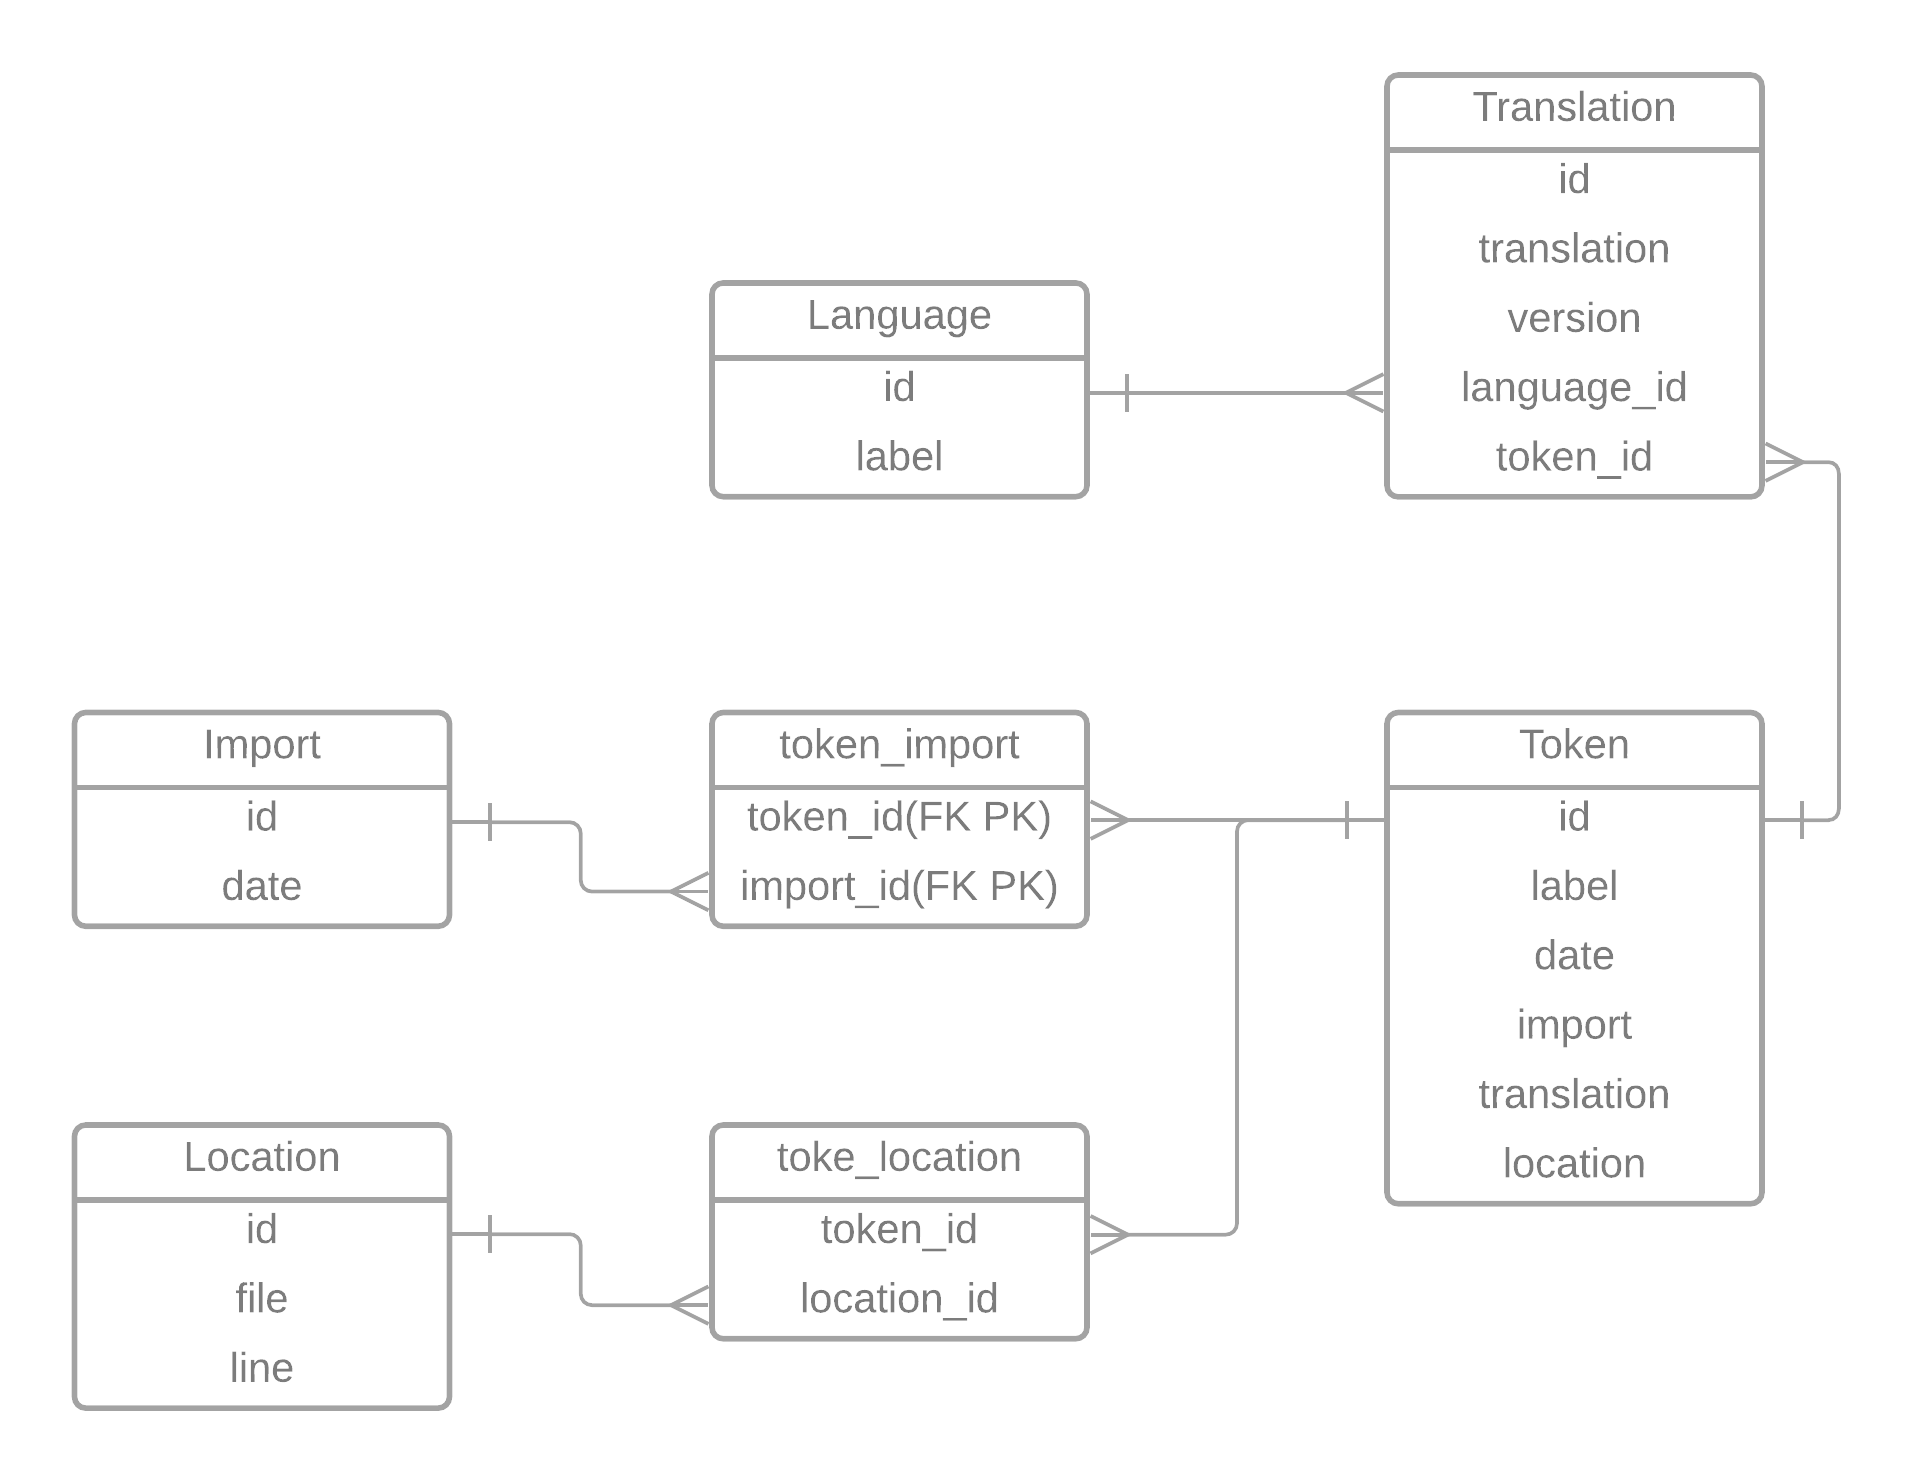
\includegraphics[width=\textwidth]{ERD_TranslationService_IST-Analyse.png}
    \caption{ERD im IST Zustand}
  \end{figure}
  \subsubsection{Finale Datenbankstruktur}\label{sec:erd:final}
  \begin{figure}[ht]
    \label{abb:erd:final}
    \centering
    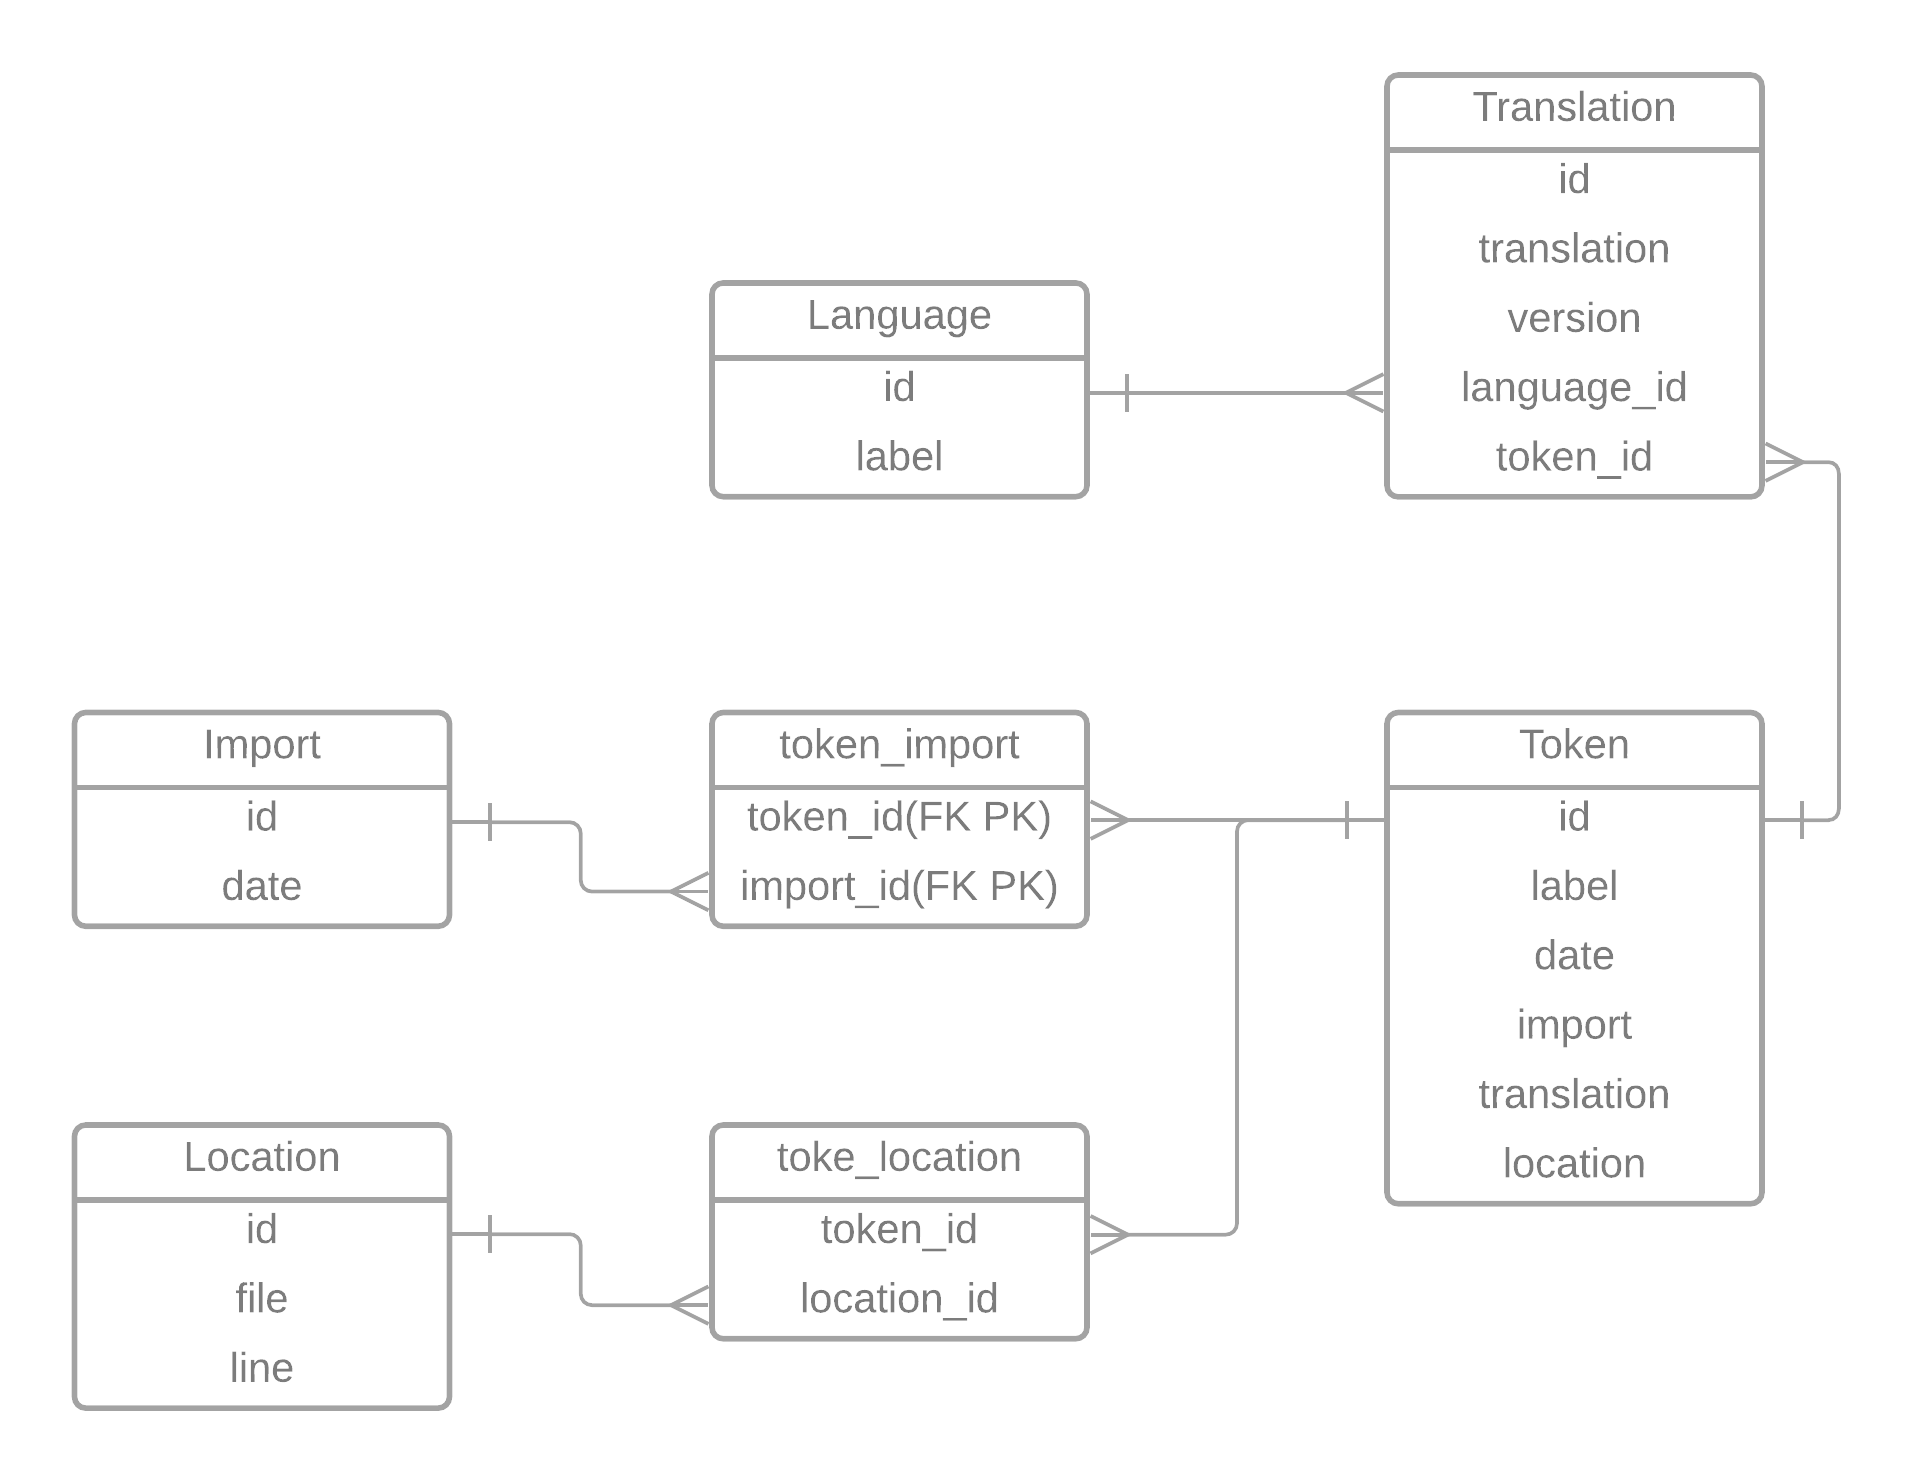
\includegraphics[width=\textwidth]{ERD_TranslationService_IST-Analyse.png}
    \caption{ERD im Soll Zustand}
  \end{figure}
  \newpage
  \subsection{UML Anwendungsfalldiagramm}\label{sec:uml:aw:new}
  \subsubsection{OkotoPOS Cash}\label{sec:uml:aw:cash}
  \subsubsection{Translationservice}\label{sec:uml:aw:ts}
  \subsection{Komponentendiagramm}\label{sec:uml:komponenten}
  \subsection{Schnittstelledokumentation}
    \label{sec:swa:ts}
  Swagger
  \subsection{Resourcen und Technologien}\label{sec:resources}
    \begin{table}[ht]
      \centering
      \begin{tabular}{| l | l |}
        1 & 2 \\
        \hline
        3 & 4\\
        \hline
      \end{tabular}
      \caption{Genutzte Resourcen}
    \end{table}
  \subsection{Testcases Translationservice}\label{sec:test:ts}
  \subsection{Testcases Translationservice}\label{sec:test:tu}
  \subsection{Iternationsplan}\label{sec:iterationplan}
  \section{Listings}
  \subsection{Many-To-Many Annotation}\label{sec:lst:mtmA}
    Token.php
  \begin{lstlisting}
    /**
     * @var Version[]|ArrayCollection
     * @ORM\ManyToMany (targetEntity="OktoCareer\TranslationService\
        Version\Version", inversedBy="tokens")
     * @ORM\JoinTable (name="token_version",
     *     joinColumns = {
     *      @ORM\JoinColumn (name="token_id", referencedColumnName="id")
     * },
     *     inverseJoinColumns={
     *      @ORM\JoinColumn (name="version_id", referencedColumnName="id")
     * }
     *     )
     */
     private $version;
  \end{lstlisting}
  Version.php
  \begin{lstlisting}
    /**
     * @var Token[]|ArrayCollection
     * @ORM\ManyToMany (targetEntity="OktoCareer\TranslationService\
        Token\Token",mappedBy="version")
     */
     private $tokens;
  \end{lstlisting}
  \subsection{Routing}\label{sec:lst:routes}
  HTTP GET Route:
  \begin{lstlisting}
    $app->get('/api/v1/version/{version}/translations/{language}'
      ,ExportTranslationAction::class);
  \end{lstlisting}
  HTTP POST Route:
  \begin{lstlisting}
    $app->post('/api/v1/version/{version}/diff/translations/{language}'
      ,CreateTranslationDiff::class);
  \end{lstlisting}
  \subsection{Beispielimplementierung einer GET-Route}\label{lst:impl:bl:GET}
  \subsection{Beispielimplementierung einer POST-Route}\label{lst:impl:bl:POST}
\end{document}